\documentclass[bachelor, och, coursework]{SCWorks}
% параметр - тип обучения - одно из значений:
%    spec     - специальность
%    bachelor - бакалавриат (по умолчанию)
%    master   - магистратура
% параметр - форма обучения - одно из значений:
%    och   - очное (по умолчанию)
%    zaoch - заочное
% параметр - тип работы - одно из значений:
%    referat    - реферат
%    coursework - курсовая работа (по умолчанию)
%    diploma    - дипломная работа
%    pract      - отчет по практике
% параметр - включение шрифта
%    times    - включение шрифта Times New Roman (если установлен)
%               по умолчанию выключен
\usepackage{subfigure}
\usepackage{tikz,pgfplots}
\pgfplotsset{compat=1.5}
\usepackage{float}

%\usepackage{titlesec}
\setcounter{secnumdepth}{4}
%\titleformat{\paragraph}
%{\normalfont\normalsize}{\theparagraph}{1em}{}
%\titlespacing*{\paragraph}
%{35.5pt}{3.25ex plus 1ex minus .2ex}{1.5ex plus .2ex}

\titleformat{\paragraph}[block]
{\hspace{1.25cm}\normalfont}
{\theparagraph}{1ex}{}
\titlespacing{\paragraph}
{0cm}{2ex plus 1ex minus .2ex}{.4ex plus.2ex}

% --------------------------------------------------------------------------%


\usepackage[T2A]{fontenc}
\usepackage[utf8]{inputenc}
\usepackage{graphicx}
\graphicspath{ {./img/} }
\usepackage{tempora}

\usepackage[sort,compress]{cite}
\usepackage{amsmath}
\usepackage{amssymb}
\usepackage{amsthm}
\usepackage{fancyvrb}
\usepackage{listings}
\usepackage{listingsutf8}
\usepackage{longtable}
\usepackage{array}
\usepackage[english,russian]{babel}

\usepackage[colorlinks=true, linkcolor=black]{hyperref}
\usepackage{url}

\usepackage{underscore}
\usepackage{setspace}
\usepackage{indentfirst} 
\usepackage{mathtools}
\usepackage{amsfonts}
\usepackage{enumitem}
\usepackage{tikz}

\usepackage{minted}
%\usemintedstyle{autumn}


\newcommand{\eqdef}{\stackrel {\rm def}{=}}
\newcommand{\specialcell}[2][c]{%
\begin{tabular}[#1]{@{}c@{}}#2\end{tabular}}

\renewcommand\theFancyVerbLine{\small\arabic{FancyVerbLine}}

\newtheorem{lem}{Лемма}

\begin{document}

% Кафедра (в родительном падеже)
\chair{теоретических основ компьютерной безопасности и криптографии}

% Тема работы
\title{Обнаружение сетевого P2P трафика методом анализа его поведения}

% Курс
\course{3}

% Группа
\group{331}

% Факультет (в родительном падеже) (по умолчанию "факультета КНиИТ")
\department{факультета КНиИТ}

% Специальность/направление код - наименование
%\napravlenie{09.03.04 "--- Программная инженерия}
%\napravlenie{010500 "--- Математическое обеспечение и администрирование информационных систем}
%\napravlenie{230100 "--- Информатика и вычислительная техника}
%\napravlenie{231000 "--- Программная инженерия}
\napravlenie{10.05.01 "--- Компьютерная безопасность}

% Для студентки. Для работы студента следующая команда не нужна.
% \studenttitle{Студентки}

% Фамилия, имя, отчество в родительном падеже
\author{Стаина Романа Игоревича}

% Заведующий кафедрой
\chtitle{д. ф.-м. н., доцент} % степень, звание
\chname{М.~Б.~Абросимов}

%Научный руководитель (для реферата преподаватель проверяющий работу)
\satitle{доцент} %должность, степень, звание
\saname{А.~В.~Гортинский}

% Руководитель практики от организации (только для практики,
% для остальных типов работ не используется)
% \patitle{к.ф.-м.н.}
% \paname{С.~В.~Миронов}

% Семестр (только для практики, для остальных
% типов работ не используется)
%\term{8}

% Наименование практики (только для практики, для остальных
% типов работ не используется)
%\practtype{преддипломная}

% Продолжительность практики (количество недель) (только для практики,
% для остальных типов работ не используется)
%\duration{4}

% Даты начала и окончания практики (только для практики, для остальных
% типов работ не используется)
%\practStart{30.04.2019}
%\practFinish{27.05.2019}

% Год выполнения отчета
\date{2022}

\maketitle

% Включение нумерации рисунков, формул и таблиц по разделам
% (по умолчанию - нумерация сквозная)
% (допускается оба вида нумерации)
% \secNumbering

%-------------------------------------------------------------------------------------------

% \begin{minted}[fontsize=\small]{MySQL}
% \end{minted}

% \begin{figure}[H]
%     \centering
%     \includegraphics[width=0.999\textwidth]{img/}
%     \caption{}
%     \label{easy_hack}
% \end{figure}

\tableofcontents

\intro
Введение

\section{Peer-to-Peer} % придумать что делать с этой секцией
\textbf{P2P} (\textbf{p}eer-\textbf{to}-\textbf{p}eer), также известные как одноранговые, децентрализованные или пиринговые сети, "--- это распределенная архитектура приложения, которая разделяет задачи между узлами (peer). Узлы имеют одинаковые привилегии в приложении и образуют сеть равносильных узлов.

Узлы делают свои ресурсы, такие как вычислительная мощность, объем диска или пропускная способность напрямую доступными остальным членам сети, без необходимости координировать действия с помощью серверов. Узлы являются одновременно поставщиками и потребителями ресурсов, в отличие от стандартной клиент-сервер модели, где поставщик и потребитель ресурсов разделены.

\subsection{История}
В то время как Р2Р системы использовались во многих доменных приложениях, архитектура популяризовалась благодаря файлообменной системе Napster, разработанной в 1999 году. Концепция вдохновила новую философию во многих областях человеческого взаимодействия. P2P технология позволяет пользователям интернета образовывать группы и коллаборации, формируя, тем самым, пользовательские поисковые движки, виртуальные суперкомпьютеры и файловые системы. Основная идея P2P систем исходит из первых принципов метода Request for Comment (RFC). Видение Всемирной паутины Тима Бернерса-Ли было близко к P2P сети, в том смысле, что каждый пользователь является активным создателем и редактором контента.

Ранней версией P2P сетей является USENET "--- распределенная система обмена сообщениями. USENET был разработан в 1979 году и представлял собой систему, обеспечивающую децентрализованную модель управления. Основа представляет собой клиент-серверную модель, предполагающую самоорганизацию группы серверов. Тем не менее сервера взаимодействуют друг с другом как равноправные узлы, распространяя информацию по всей сети USENET.

В мае 1999 года, в Интернет с более чем миллионом пользователей, Шон Фэннинг внедрил приложение файлообменник Napster. Napster стал началом P2P сети, такой какую мы знаем её сейчас, пользователи участвуют в создании виртуальной сети, полностью независимой от физической, без администрирования и каких-либо ограничений.

\section{Архитектура} % надо подумать над оформлением ссылок
P2P сеть строится вокруг понятия равноправных узлов "--- клиенты и серверы одинаково взаимодействуют с другими узлами сети. Такая модель построения сети отличается от модели клиент-сервер, где взаимодействие идет с центральным сервером. 
На рисунке \ref{ris:image1} а) изображены архитектура клиент-сервера и б) архитектура P2P. Типичным примером передачи файла в модели клиент-сервер является File Transfer Protocol (FTP), в котором программы клиента и сервера разделены: клиент инициирует передачу, а сервер отвечает на запросы. 

\begin{figure}[h]
    \begin{minipage}[h]{0.49\linewidth}
        \center{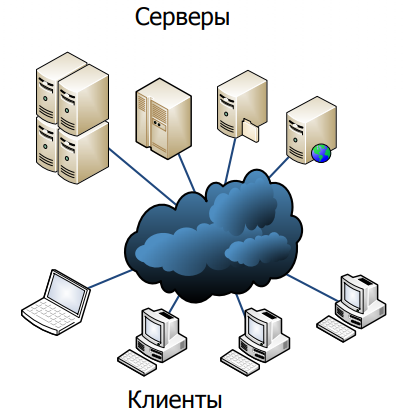
\includegraphics[width=0.75\linewidth]{arch_client-server.png} \\ а)}
    \end{minipage}
    \hfill
    \begin{minipage}[h]{0.49\linewidth}
        \center{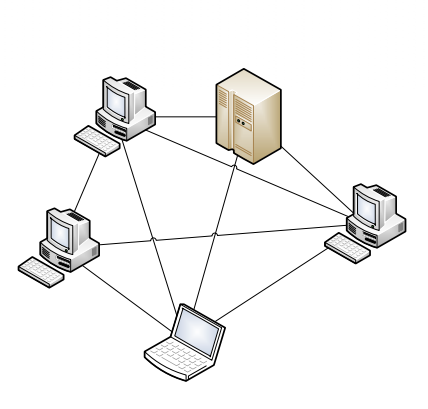
\includegraphics[width=0.75\linewidth]{arch_p2p.png} \\ б)}
    \end{minipage}
    \caption{Архитектура клиент-сервера и P2P}
    \label{ris:image1}
\end{figure}

\subsection{Базовые элементы P2P сетей}
\subsubsection{Узел P2P сети}
\textbf{Узел (Peer)} "--- фундаментальный составляющие блок любой одноранговой сети. Каждый узел имеет уникальный идентификатор и принадлежит одной или нескольким группам. Он может взаимодействовать с другими узлами как в своей, так и в других группах.

Виды узлов:
\begin{itemize}
    \item \textbf{Простой узел}. Обеспечивает работу конечного пользователя, предоставляя ему сервисы других узлов и	
    обеспечивая предоставление ресурсов пользовательского компьютера другим	участникам сети.
    \item \textbf{Роутер}. Обеспечивает механизм взаимодействия между узлами, отделёнными от сети брандмауэрами или NAT-системами.	
\end{itemize}

\subsubsection{Группа узлов}
\textbf{Группа узлов} "--- набор узлов, сформированный для решения общей задачи или достижения общей цели. Могут предоставлять членам своей группы такие наборы сервисов, которые недоступны узлам, входящим в другие группы.

Группы узлов могут разделяться по следующим признакам:
\begin{itemize}
    \item приложение, ради которого они объединены в группу;
    \item требования безопасности;
    \item необходимость информации о статусе членов группы.
\end{itemize}

\subsubsection{Сетевой транспорт}
\textbf{Конечные точки (Endpoints)} "--- источники и приёмники любого массива данных передаваемых по сети.

\textbf{Пайпы (Pipes)} "--- однонаправленные, асинхронные виртуальные коммуникационные каналы, соединяющие две или более конечные точки.

\textbf{Сообщения} "--- контейнеры информации, которая передаётся через пайп от одной конечной точки до другой.

\subsection{Маршрутизация}
P2P сети обычно реализуют некоторую форму виртуальной сети, наложенную поверх физической сети, где узлы образуют подмножество узлов в физической сети. Данные по-прежнему обмениваются непосредственно над базовой TCP/IP сетью, а на прикладном уровне узлы имеют возможность взаимодействовать друг с другом напрямую, с помощью логических связей. Наложение используется для индексации и обнаружения узлов, что позволяет системе P2P быть независимой от физической сети. На основании того, как узлы соединены друг с другом внутри сети, и как ресурсы индексированы и расположены, сети классифицируются на \textbf{неструктурированные} и \textbf{структурированные} (или как их \textbf{гибрид}).

\subsubsection{Неструктурированные сети}
Неструктурированная Р2Р сеть не формирует определенную структуру сети, а случайным образом соединяет узлы друг с другом. Так как не существует глобальной структуры формирования сети, неструктурированные сети легко организуются и доступны для локальных оптимизаций. Кроме того, поскольку роль всех узлов в сети одинакова, неструктурированные сети являются весьма надежными в условиях, когда большое количество узлов часто подключаются к сети или отключаются от нее.

Однако, из-за отсутствия структуры, возникают некоторые ограничения. В частности, когда узел хочет найти нужный фрагмент данных в сети, поисковый запрос должен быть направлен через сеть, чтобы найти как можно больше узлов, которые обмениваются данными. Такой запрос вызывает очень высокое количество сигнального трафика в сети, требует высокой производительности, и не гарантирует, что поисковые запросы всегда будут решены.

\subsubsection{Структурированные сети}
В структурированных Р2Р сетях наложение организуется в определенную топологию, и протокол гарантирует, что любой узел может эффективно участвовать в поиске файла или ресурса, даже если ресурс использовался крайне редко.

Наиболее распространенный тип структурированных сетей P2P реализуется распределенными хэш-таблицами (DHT), в котором последовательное хеширование используется для привязки каждого файла к конкретному узлу. Это позволяет узлам искать ресурсы в сети, используя хэш-таблицы, хранящих пару ключ-значение, и любой участвующий узел может эффективно извлекать значение, связанное с заданным ключом.

Тем не менее, для эффективной маршрутизации трафика через сеть, узлы структурированной сети должны обладать списком соседей, которые удовлетворяют определенным критериям. Это делает их менее надежными в сетях с высоким уровнем оттока абонентов (т.е. с большим количеством узлов, часто подключающихся к сети или отключающихся от нее).

\subsubsection{Гибридные модели}
Гибридные модели представляют собой сочетание Р2Р сети и модели клиент-сервер. Гибридная модель должна иметь центральный сервер, который помогает узлам находить друг друга. Есть целый ряд гибридных моделей, которые находят компромисс между функциональностью, обеспечиваемой структурированной сетью модели клиент-сервер, и равенством узлов, обеспечиваемой чистыми одноранговыми неструктурированными сетями. В настоящее время гибридные модели имеют более высокую производительность, чем чисто неструктурированные или чисто структурированные сети.

\subsection{Безопасность}
Как и любой другой форме программного обеспечения, P2P приложения могут содержать уязвимости. Особенно опасно для P2P программного обеспечения, является то, что Р2Р приложения действуют и в качестве серверов и в качестве клиентов, а это означает, что они могут быть более уязвимы для удаленных эксплоитов.

\subsubsection{Маршрутизационные атаки}
Поскольку каждый узел играет роль в маршрутизации трафика через сеть, злоумышленники могут выполнять различные <<маршрутизационные атаки>>, или атаки отказа в обслуживании. Примеры распространенных атак маршрутизации включают в себя <<неправильная маршрутизация поиска>>, когда вредоносные узлы преднамеренно пересылают запросы неправильно или возвращают ложные результаты, <<неправильная маршрутизация обновления>>, когда вредоносные узлы изменяют таблицы маршрутизации соседних узлов, посылая им ложную информацию, и <<неправильная маршрутизация разделения сети>>, когда новые узлы подключаются через вредоносный узел, который помещает новичков в разделе сети, заполненной другими вредоносными узлами.

\subsubsection{Поврежденные данные и вредоносные программы}
Распространенность вредоносных программ варьируется между различными протоколами одноранговых сетей. Исследования, анализирующие распространение вредоносных программ по сети P2P обнаружили, например, что 63\% запросов на загрузку по сети Limewire содержали некоторую форму вредоносных программ, в то время как на OpenFT только 3\% запросов содержали вредоносное программное обеспечение. Другое исследование анализа трафика в сети Kazaa обнаружили, что 15\% от 500 000 отобранных файлов, были инфицированы одним или несколькими из 365 различных компьютерных вирусов.

Поврежденные данные также могут быть распределены по P2P-сети путем изменения файлов, которые уже были в сети. Например, в сети FastTrack, RIAA удалось внедрить фальшивые данные в текущий список загрузок и в уже загруженные файлы (в основном файлы MP3). Файлы, инфицированные вирусом RIAA были непригодны впоследствии и содержали вредоносный код. Следовательно, P2P сети сегодня внедрили огромное количество механизмов безопасности и проверки файлов. Современное хеширование, проверка данных и различные методы шифрования сделали большинство сетей, устойчивыми к практически любому типу атак, даже когда основные части соответствующей сети были заменены фальшивыми или нефункциональными узлами.

\subsection{Отказоустойчивость и масштабируемость сети}
Децентрализованность Р2Р сетей повышает их надежность, так как этот метод взаимодействия устраняет ошибку единой точки разрыва, присущую клиент-серверным моделям. С ростом числа узлов, объем трафика внутри системы увеличивается, масштаб сети также увеличивается, что приводит к уменьшению вероятности отказа. Если один узел перестанет функционировать должным образом, то система в целом все равно продолжит работу. В модели клиент-сервер, с ростом количества пользователей, уменьшается количество ресурсов выделяемых на одного пользователя, что приводит к риску возникновения ошибок.

\subsection{Распределенное хранение и поиск}
Возможность резервного копирования данных, восстановление и доступность приводят как и к преимуществами так и к недостаткам Р2Р сетей. В централизованной сети, только системный администратор контролирует доступность файлов. Если администраторы решили больше не распространять файл, его достаточно удалить с серверов, и файл перестанет быть доступным для пользователей. Другим словами, клиент-серверные модели имеют возможность управлять доступностью файлов. В Р2Р сети, доступность контента определяется степенью его популярности, так как поиск идет по всем узлам, через которые файл проходил. То есть, в Р2Р сетях нет централизованной власти, как системный администратор в клиент-серверном варианте, а сами пользователи определяют уровень доступности файла.

\section{Применение}
В Р2Р сетях, пользователи передают и используют контент сети. Это означает, что в отличие от клиент-серверных сетей, скорость доступа к данным возрастает с увеличением числа пользователей, использующих этот контент. На этой идее построен протокол Bittorrent "--- пользователи скачавшие файл, становятся узлами и помогают другим пользователям скачать файл быстрее. Эта особенность является главным преимуществом Р2Р сетей.

Множество файлообменных систем, таких как Gnutella, G2 и eDonkey популяризовали Р2Р технологии:
\begin{itemize}
    \item Пиринговые системы распространения контента.
    \item Пиринговые системы обслуживания, например повышение производительности, в частности Correli Caches.
    \item Публикация и распространение программного обеспечения (Linux, видеоигры).
\end{itemize}

В связи децентрализованностью доступа к данным в Р2Р сетях возникает проблема нарушения авторских прав. Компании, занимающиеся разработкой Р2Р приложений часто принимают участие в судебных конфликтах. Самые известные судебные дела это Grokster против RIAA и MGM Studios, Inc. против Grokster Ltd., где в обоих случаях технологии файлообменных систем признавались законными.

\section{Описание программы}
В данной работе был разработан \textbf{сниффер} "--- анализатор сетевого трафика. Программа выводит на экран информацию о перехваченных пакетах таких сетевых протоколов как \textit{Ethernet}, \textit{IPv4}, \textit{TCP} и \textit{UDP}. Дополнительно последний вывод программы сохраняется в текстовый файл.

\subsection{Руководство}
Запуск программы возможен \underline{только} на ОС \textit{Linux} с установленным языком программирования \textit{Python3}.

Для работы с программой необходимо запустить \textit{window.py} с правами администратора:
\begin{minted}[fontsize=\small]{bash}
    sudo ./window.py
\end{minted}
После открытия окна необходимо нажать кнопку <<Старт>>.

\subsection{Принцип работы}
\subsubsection{Интерфейсная часть программы}
При запуске \textit{window.py} создаётся \textbf{сокет} "--- программный интерфейс для обеспечения обмена данными между процессами. \underline{Через него проходит весь} \\ \underline{сетевой трафик на той виртуальной машине, на которой он находится}. % !

\begin{minted}[fontsize=\small]{python3}
    conn = socket.socket(socket.AF_PACKET, socket.SOCK_RAW, socket.ntohs(3))
\end{minted}

Далее открывается окно интерфейса, в котором создаются необходимые виджеты: кнопка <<Старт>> и текстовое поле для вывода информации. Нажатие кнопки <<Старт>> вызывает функцию \textit{sniff}, которая вызывает функцию \textit{main} из \textit{sniffer.py}. Результат выполнения функции \textit{main} "--- информация о перехваченном пакете. Данная информация выводится в текстовое поле интерфейса и в текстовый файл \textit{out.txt}. Дополнительно выводится системное время "--- когда был получен или отправлен очередной пакет. 

\begin{minted}[fontsize=\small]{python3}
    def sniff(self):
    out = sniffer.main(conn)
    out.insert(0, str(datetime.now().strftime('%H:%M:%S')) + ":")
    for s in out:
        file.write(s + '\n')
        self.output.insert('end', s + '\n')
    root.after(300, self.sniff)  # сканирование каждые 0.3 сек
\end{minted}

Функция \textit{sniff} вызывает рекурсивно саму себя каждые 0.3 секунды, то есть сканирование происходит раз в 0.3 секунды. 

\subsubsection{Основная функция программы}
Основная функция \textit{main} получает данные с сокета и затем анализирует и форматирует их с помощью вспомогательных функций. Она позволяет получить информацию о \textit{Ethernet}, \textit{IPv4}, \textit{TCP} и \textit{UDP} пакетах. Стоит отметить, что данные, передающиеся в пакетах, не выводятся, потому что они представлены в виде массива байт (данные могут быть зашифрованы, поэтому извлечь из них информацию затруднительно). 

\subsubsection{Определение P2P трафика}
Если был получен \textit{TCP} или \textit{UDP} пакет, то проверяются порты источника и назначения. В списке пар порт-приложение \textit{LIST_p2p} находится информация о используемых портах некоторых P2P приложений, а именно:

\begin{itemize}
    \item BitTorrent;
    \item Direct Connect;
    \item eDonkey;
    \item FastTrack;
    \item Yahoo;
    \item Napster;
    \item Gnutella;
    \item AIM;
    \item Skype;
    \item Steam;
    \item Hamachi;
    \item Radmin VPN;
\end{itemize}

Если был обнаружен порт, который есть в данном списке, то в информацию о пакете дополнительно заносится строка <<Обнаружен P2P трафик (методом анализирования портов)>>.

Конечно же, данный метод не даёт гарантии обнаружения и не позволяет однозначно идентифицировать приложение и тип данных, передающихся по P2P сети.

\subsubsection{Тестирование программы}
Для тестирования программы использовался \textit{Skype} "--- приложение для проведения аудио и видео звонков, а также обмена текстовыми сообщениями. Звонки происходят с помощью P2P. На \ref{ris:test_skype} рисунке показана работа программы во время активного аудио звонка в Skype. С помощью метода анализирования портов был обнаружен P2P трафик.

\begin{figure}[H]
    \centering
    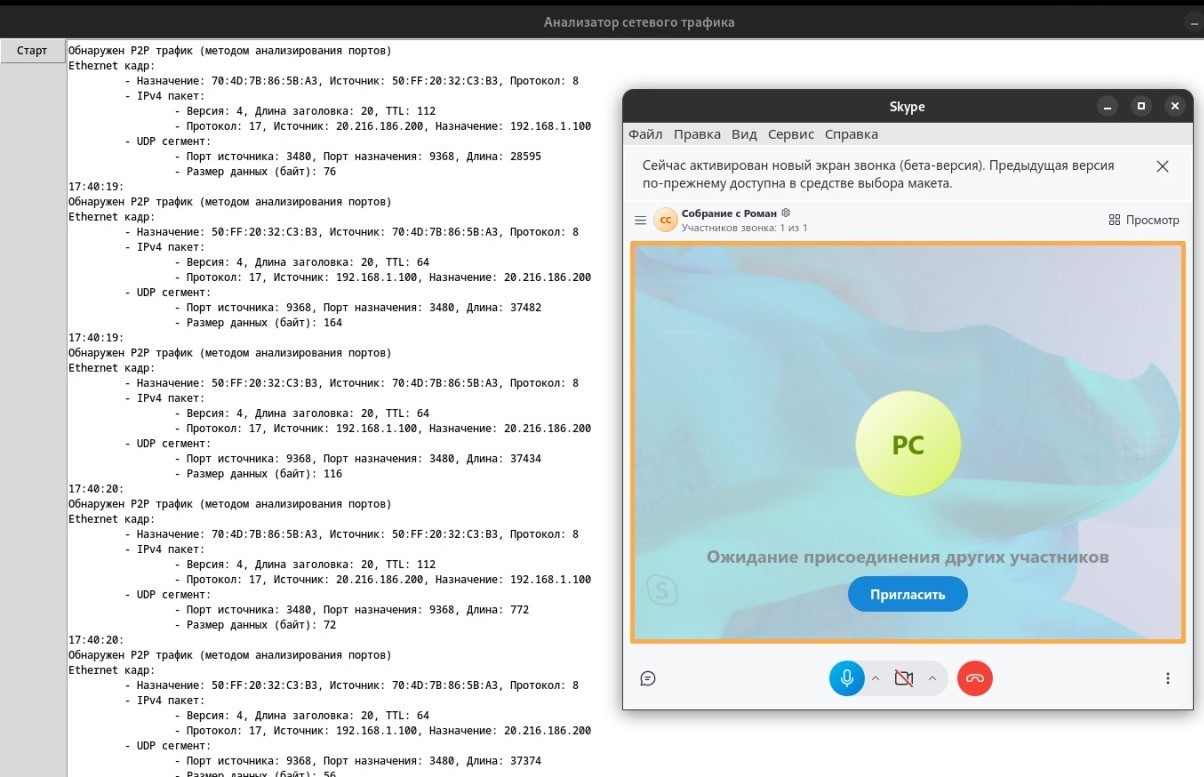
\includegraphics[width=1\textwidth]{test1.jpg}
    \caption{Тестирование работы программы при запущенном звонке в Skype}
    \label{ris:test_skype}
\end{figure}

В данном примере обнаружен порт 3480, который присутствует в списке отслеживаемых портов \textit{LIST_p2p}.


\conclusion
Заключение

\bibliographystyle{gost780uv}
\bibliography{thesis}


\end{document}
